% \documentclass[12pt,fleqn]{beamer}

% \usepackage{amsmath, amsthm, amssymb} %math expressions, theoreme/lemma, math symbols
% \usepackage{mathtext} %russian letters in formulas

% % fonts and lang
% %\usepackage[T1,TS1,T2A]{fontenc}
% \usepackage{cmap}
% \usepackage[T1, T2A]{fontenc}
% \usepackage[utf8]{inputenc}
% \usepackage[english, russian]{babel}

% % formatting
% % \usepackage{geometry} %customize page layout
% % \geometry{left = 3cm}
% % \geometry{right = 1cm}
% % \geometry{top = 1.5cm}
% % \geometry{bottom = 2cm}

% \usepackage{setspace} %set space between lines
% \usepackage{indentfirst} %indent first pagearagraph after section header

% \usepackage{tocloft} %control table of contents, figures

% \usepackage{graphicx}

% \usepackage{hhline}

% \usepackage{caption}

% \usepackage{subcaption}

% \usepackage[shortlabels]{enumitem}
% \setlist{nolistsep, itemsep=0.1cm, parsep=0pt, leftmargin=1.5cm}

% \usepackage{multirow}

% \usepackage{algorithm}
% \usepackage{algpseudocode}

%%%%%%%%%%%%%%%% что - то про dvips
% latex yourfile.tex
% dvips yourfile.dvi
% ps2pdf yourfile.ps
%aspectratio=169
\documentclass[unicode, t, 11pt]{beamer}% [t], [c], или [b] --- вертикальное выравнивание на слайдах (верх, центр, низ)
%\documentclass[aspectratio=169]{beamer} % Соотношение сторон

%%% Работа с русским языком
\usepackage{cmap}					% поиск в PDF
\usepackage{mathtext} 				% русские буквы в формулах
% \usepackage[T2A]{fontenc}			% кодировка
\usepackage[T1, T2A]{fontenc}
\usepackage[utf8]{inputenc}			% кодировка исходного текста
\usepackage[english,russian]{babel}	% локализация и переносы

% %% Beamer по-русски
% \newtheorem{rtheorem}{Теорема}
% \newtheorem{rproof}{Доказательство}
% \newtheorem{rexample}{Пример}
\usepackage{amsmath, amsfonts, amssymb, amsthm, mathtools} % AMS
\usepackage{icomma} % "Умная" запятая: $0,2$ --- число, $0, 2$ --- перечисление

%% Номера формул
%\mathtoolsset{showonlyrefs=true} % Показывать номера только у тех формул, на которые есть \eqref{} в тексте.
%\usepackage{leqno} % Нумерация формул слева

%%% Работа с картинками
\usepackage{graphicx}  % Для вставки рисунков
%\graphicspath{{presentation/images/}}  % папки с картинками
\setlength\fboxsep{3pt} % Отступ рамки \fbox{} от рисунка
\setlength\fboxrule{1pt} % Толщина линий рамки \fbox{}
\usepackage{wrapfig} % Обтекание рисунков текстом

%%% Работа с таблицами
\usepackage{array,tabularx,tabulary,booktabs} % Дополнительная работа с таблицами
\usepackage{longtable}  % Длинные таблицы
\usepackage{multirow} % Слияние строк в таблице

%%% Программирование
\usepackage{etoolbox} % логические операторы

%%% Другие пакеты
\usepackage{lastpage} % Узнать, сколько всего страниц в документе.
\usepackage{soul} % Модификаторы начертания
\usepackage{csquotes} % Еще инструменты для ссылок
%\usepackage[style=authoryear,maxcitenames=2,backend=biber,sorting=nty]{biblatex}
\usepackage{multicol} % Несколько колонок

%%% Картинки
\usepackage{tikz} % Работа с графикой
% \usepackage{pgfplots}
% \usepackage{pgfplotstable}

\usepackage{enumerate}
\usepackage{enumitem}
\setlist[itemize]{noitemsep, topsep=0pt}

\usepackage{caption}
\DeclareCaptionFont{tiny}{\tiny}
\captionsetup{belowskip=0pt}
\setlength{\belowcaptionskip}{-10pt}

\newlength{\mylen}

\usepackage{tabularx}

%\usefonttheme{professionalfonts} % using non standard fonts for beamer
\usefonttheme{serif} % default family is serif

\setbeamertemplate{footline}[frame number]







%%%%%%%%%%%%%%%%%%%%%%%%%%%%%%%%%%%%%%%%%%%%%%%%%%%%%%%%%%%%%%%%%%%%%%%%%%%%%%%%%%%%
\title{
	{\footnotesize\color{black}Московский государственный университет имени М.В.Ломоносова\\
    Факультет Вычислительной Математики и Кибернетики\\
    Кафедра Суперкомпьютеров и Квантовой Информатики\\}
    \vspace{\baselineskip}
    {\LARGEРазработка метода прогнозирования слабой масштабируемости суперкомпьютерных приложений}
}
%\subtitle{SUBTITLE}
\author{\footnotesizeСтудент: Мокров К.С., 423 группа\\
		Науч. руководитель: к.ф-м.н.,
		в.н.с. НИВЦ МГУ\\
		Антонов Александр Сергеевич}

\date{
\includegraphics[height=0.8cm]{./images/MSU}\\
	  \scriptsize
	  Москва\\
	  2020 г.}
%\logo{
\includegraphics[height=1.5cm]{./images/MSU}}
%%%%%%%%%%%%%%%%%%%%%%%%%%%%%%%%%%%%%%%%%%%%%%%%%%%%%%%%%%%%%%%%%%%%%%%%%%%%%%%%%%%%


\begin{document}

	\frame[plain]{\titlepage}	% Титульный слайд
	% СКАЗТЬ
	% ПРО
	% УНИВЕРСАЛЬНОСТЬ
	% Требование универсальности и отсутствия информации о коде, алгоритме И СИСТЕМЕ НА КОТОРОЙ ПРОИЗВОДЯТСЯ ЗАПУСКИ
	\section{Введение}
		\begin{frame}
		\footnotesize
		\frametitle{\insertsection}
		\begin{itemize}[label = \(\bullet\)]
		\item Масштабируемость - свойство параллельной программы, характеризующее зависимость изменения всей совокупности динамических характеристик работы этой программы от множества параметров её запуска.
		%\item Масштабируемость - ключевая характеристика параллельных программ. Крайне важно учитывать её во время исследования свойств этих программ или в процессе их разработки.
		%сказать про разные виды масштабируемости и что значит хорошая масштабируемость для каждого из них
		\item Не всегда возможно получить в распоряжение большое количество узлов, чтобы увидеть характер изменения различных динамических характеристик приложения с ростом числа используемых ресурсов системы, при увеличении размера задачи.
		%, или ожидание этого может занять непозволительно много времени, например, авторы статьи \cite{log_main} утверждают, что в худшем случае время ожидания выделения необходимого количества узлов растёт экспоненциально с ростом количества запрашиваемых ресурсов. Но ведь 
		\item Возможность решать задачи больших размеров за разумное время, используя большое количество узлов, является главным преимуществом суперкомпьютерных систем, поэтому необходимо, чтобы приложение было хорошо масштабируемо.
		%Обычно пользователь может выполнить задачу на небольшой конфигурации быстрее, чем запустить на большом количестве узлов. Исходя из этого, 
		\item Актуальна задача прогнозирования масштабируемости приложения на большие конфигурации вычислительной системы, основываясь только на данных, полученных из множественных запусков на малых конфигурациях.

		%В данной работе предлагается механизм решения поставленной задачи в условиях слабой масштабируемости суперкомпьютерных приложений.    --- СКАЗАТЬ ПОЧЕМУ
		\end{itemize}
		\end{frame}

	\section{Постановка задачи}
		\begin{frame}
			\frametitle{\insertsection}
			\begin{itemize}[label=\(\bullet\)]
				\item Исследовать возможные подходы к предсказанию масштабируемости.
				\item Реализовать метод, предсказывающий слабую масштабируемость суперкомпьютерных приложений на основе экспериментальных данных.
				\item Проверить применимость метода на различных приложениях, собрав экспериментальную базу и оценив точность предсказаний.
			\end{itemize}
		\end{frame}

	\section{Обзор существующих подходов к предсказанию масштабируемости}
		\begin{frame}
			\frametitle{\insertsection}

			\begin{columns}
				\setlength{\mylen}{0.45\textwidth}
	 			\begin{column}{\mylen}
					\setbeamercovered{transparent}
					\begin{itemize}[label = \(\bullet\)]
						\item<1> Линейная регрессия.
						\item<2> Методы машинного обучения.
						\item<3> Симуляция исполнения программы.
						\item<4> Коллаборативная фильтрация.
					\end{itemize}
				\end{column}
				\begin{column}{\dimexpr\textwidth-\mylen}	
					\footnotesize
					\only<1>{
					\begin{itemize}
						\item[\(\textbf{+}\)] Модель простая, легко искать неизвестные параметры.
						\item[\(\textbf{+}\)] Для поиска параметров не требуется большое число запусков.
						\item[\(\textbf{+}\)] Точность предсказаний либо сопоставима, либо даже лучше, чем у других методов
						\item[\(\textbf{---}\)] Далеко не всегда простая модель может описать поведение рассматриваемой величины из-за её нелинейного характера изменения
					\end{itemize}
					}
					\only<2>{
					\begin{itemize}
						\item[\(\textbf{+}\)] Способны уловить сложные аспекты взаимодействия между архитектурой суперкомпьютера и исследуемыми программами.
						\item[\(\textbf{+}\)] Есть возможность работать при наличии неинформативных, зашумлённых входных данных.
						\item[\(\textbf{---}\)] Для обучения необходимо провести большое число запусков приложения.
						\item[\(\textbf{---}\)] Относительно высокая вычислительная стоимость процесса обучения как по времени, так и по памяти.
						\item[\(\textbf{---}\)] Чёрный ящик - невозможно объяснить ответ.
					\end{itemize}
					}
					\only<3>{
					\begin{itemize}
						\item[\(\textbf{+}\)] Сбор трасс исполнения приложения и его профилирование может быть произведено на одной машине для последующей симуляции исполнения на другой.
						\item[\(\textbf{---}\)] Часто требует для своей работы наличия информации о структуре программы и подробных технических характеристик используемой системы.
						\item[\(\textbf{---}\)] Сложно реализовать.
					\end{itemize}
					}
					\only<4>{
					\begin{itemize}
						\item[\(\textbf{+}\)] Давно используется в рекомендательных системах, где хорошо себя зарекомендовала.
						\item[\(\textbf{---}\)] Для построения точных прогнозов необходимо провести много тестирований программы и иметь доступ к большим наборам параметров запуска программы и динамических характеристик исполнения.
					\end{itemize}
					}
				\end{column}
			\end{columns}
		\end{frame}

	\section{Описание разработанного метода}
		\subsection{Экстраполирующая функция и оценка ошибок предсказаний}
			\begin{frame}
				\frametitle{\insertsection}
					\framesubtitle{\insertsubsection}
					% {
					% %\setbeamercolor{block title}{bg=red!30,fg=blue}
					% \setbeamertemplate{blocks}[rounded][shadow]
					% \setbeamercolor{block body}{bg=structure!10, fg=black}
					%\begin{block}{fdfsf}
					\begin{itemize}[label = \(\bullet\)]
						\item С помощью линейной регрессии строятся предсказания значений динамических характеристик на \(p_{target}\) процессах, использую эмпирические данные, полученные из нескольких запусков на \(\mathbb{Q} = \{q_1,\ldots, q_n\},\ q_1 < q_2 < \ldots < q_n < p_{target}\) процессах.
						%\end{block}
						%\begin{block}{}
						\item Предиктор - функция от параметров запуска и количества используемых процессов: \(\label{main_formula}DF = \hat{DF} + error = F(x_1, x_2, \ldots, x_n, p) + error\)
						%\end{block}
						%\begin{block}{}
						\item Для нахождения оптимальных значений параметров используется метод наименьших квадратов, он минимизирует:

						{\small\(SSE = |f(w, g(X)) - y|_2 = \sum_{i = 1}^{N}{(f(w, g_i(X)) - y_i)^2 \xrightarrow[w]{} min}\)}
						%\end{block}
					\end{itemize}
			\end{frame}
			\begin{frame}
				\frametitle{\insertsection}
					\framesubtitle{\insertsubsection}
					\begin{itemize}[label = \(\bullet\)]
						\item Использование LSM эквивалентно минимизации абсолютной ошибки \(error\). Но для оценки качества предсказаний принято использовать относительную ошибку.
						%СКАЗАТЬ ПОЧЕМУ
						\begin{tikzpicture}
							\draw [thick, ->] 
							(1,0.25) -- (0,0);
							\draw [thick, ->]
							(1,0.25) -- (2,0);
							\draw
							(1,0.25) node[above] {\(RE = \frac{|DF - \hat{DF}|}{DF}\)};
							%(0,0) node[left] {\(RE_{norm} = \frac{|error|}{\only<1>{\color{black}DF}\only<2->{\color{red}DF}}\)}
							\onslide<2->{
							\draw
							(0,0) node[left] {\(RE_{norm} = \frac{|error|}{\color{red}DF}\)};
							}
							%(0,0) node[left] {\(RE_{norm} = \frac{|error|}{\only<1>{\color{black}DF}\only<2->{\color{red}DF}}\)}
							\onslide<3->{
							\draw
							(2,0) node[right] {\(RE_{log}= 2^{|{\color{green}error}|} - 1\)};
							}
						\end{tikzpicture}
						\item
					\onslide<2->{Относительная ошибка зависит не только от минимизируемой с помощью метода наименьших квадратов ошибки, но и от значения динамической характеристики.}
					\onslide<3->{Поэтому был применён один из методов преодоления этой проблемы - приближение аппроксимируемой величины в логарифмическом масштабе:
					\(\log{(DF)} = \log{\hat{(DF)}} + error\)}
					\onslide<4->{, где
					\(\log{\hat{(DF)}} = w_{1} \cdot \log{(p)} + w_{2} \cdot \log{(N)} + w_{3} \cdot \log{(p)} \cdot \log{(N)}\)}
					\end{itemize}
					% Здесь за \(N\) обозначен размер задачи, а за \(p\) количество процессов, на которых эта задача запускается. Несмотря на наличие логарифмов, статистически это всё ещё линейная модель, поскольку она линейна относительно неизвестных параметров, поэтому можно использовать обширную статистическую теорию линейных моделей, в том числе поиск коэффициента с помощью метода наименьших квадратов.

					% \begin{tikzpicture}
					% 	\draw [thick, ->] 
					% 	(2,0.5) -- (0,0);
					% 	\draw [thick, ->]
					% 	(2,0.5) -- (4,0);
					% 	\draw
					% 	(0,0) node[left] {\(RE_{norm} = \frac{|error|}{\only<1>{\color{black}DF}\only<2-3>{\color{red}DF}}\)}
					% 	(2,0.5) node[above] {\(RE = \frac{|DF - \hat{DF}|}{DF}\)}
					% 	(4,0) node[right] {\(RE_{log}= 2^{|{\only<1-2>{\color{black}error}\only<3>{\color{green}error}}|} - 1\)};						
					% \end{tikzpicture}
					% Относительная ошибка зависит не только от минимизируемой с помощью метода наименьших квадратов ошибки, но и от значения динамической характеристики. Поэтому был применён один из способов преодоления этой проблемы - приближение величины в логарифмическом масштабе:
					% \(\log{(DF)} = \log{\hat{(DF)}} + error = \beta_{1} \cdot \log{(p)} + \beta_{2} \cdot \log{(N)} + \beta_{3} \cdot \log{(p)} \cdot \log{(N)} + error\)
			\end{frame}

		% \subsection{Выбор конфигураций и проведение запусков}
		% 	\begin{frame}
		% 		\frametitle{\insertsection}
	 % 			\framesubtitle{\insertsubsection}
	 % 			\begin{itemize}[label=\(\bullet\)]
		% 			\item Для того чтобы исследовать слабую масштабируемость должно быть \textbf{заранее известно}, какие параметры запуска отвечают за определение размера задачи и как именно сложность работы программы зависит от этих самых параметров.
		% 			% Зная на скольких процессах требуется запустить задачу, сложность программы и используя соотношение \eqref{weak_sc}, можно установить, какая должна быть сложность задачи и определяющие её параметры запуска программы. Тогда процессы из множества \(\mathbb{Q}\) вместе с соответствующими им параметрами запуска будем называть тестовыми конфигурациями, а конфигурации, на которых будет оцениваться качество предсказаний метода - целевыми.
		% 			\item При сборе тестовых данных необходимо прежде всего определить тестовые конфигурации запусков. Для этого нужно узнать, сколько доступно процессов - \(p_{max}\), составить множество \[\mathbb{Q} = \{q_{i + 1} - q_{i} = const,\ i = \overline{1,n - 1};\ q_n = p_{max}\}\] и определить соответствующие параметры запуска.
		% 			% \item Выбор тестовых конфигураций: установить, сколько доступно процессов - \(p_{max}\), составить множество \[\mathbb{Q} = \{q_{i + 1} - q_{i} = const,\ i = \overline{1,n - 1};\ q_n = p_{max}\}\] и определить соответствующие параметры запуска.
		% 			% Сказать про то как я это делал, про очередь test
		% 		\end{itemize}
		% 	\end{frame}
		% 	\begin{frame}
		% 		\frametitle{\insertsection}
	 % 			\framesubtitle{\insertsubsection}
	 % 			\begin{itemize}[label=\(\bullet\)]
		% 			\item Для нескольких запусков приложения с фиксированными параметрами наблюдается разброс значений динамических характеристик \(\Rightarrow\) необходимо проводить \textbf{множественные запуски}(5-7) приложения для каждой конкретной конфигурации.
		% 			% Это можно объяснить различным размещением процессов на узлах вычислительной системы, различной степенью загруженности коммуникационной сети во время работы приложения. ||| 
		% 			% Чтобы затем в зависимости от рассматриваемой динамической характеристики выбрать достигнутый максимум или минимум значения динамической характеристики среди запусков с идентичными параметрами запуска.
		% 			\item В качестве динамических характеристик, для которых строятся предсказание масштабируемости, выбраны время выполнения программы и её производительность. Для набора запусков с идентичными конфигурациями выбирается \textbf{минимум времени исполнения и максимум производительности} среди всех запусков набора.
		% 			% Для двух из пяти выбранных программ производительность измеряется в GFlops, ещё для одной в MTeps, а для остальных двух рассматривается только время выполнения, так как точно посчитать производительность не представляется возможным.
		% 		\end{itemize}
		% 	\end{frame}
		\subsection{Общая схема работы метода}
		\begin{frame}
			\frametitle{\insertsection}
	 		\framesubtitle{\insertsubsection}
	 		\begin{enumerate}[label=\arabic*)]
				\item Определение набора тестовых конфигураций.
				\item Проведение запусков с этими конфигурациями.
				\item Извлечение из результатов запусков необходимых для поиска неизвестных коэффициентов модели данных, для идентичных конфигураций выбор минимума времени / максимума производительности исполнения.
				\item Использование метода наименьших квадратов для подбора коэффициентов линейной регрессии.
				\item Построение предсказаний значений динамических характеристик для заданного множества целевых запусков с помощью построенной модели.
			\end{enumerate}
		\end{frame}

	\section{Экспериментальная проверка применимости метода}
	% СКАЗАТЬ ПРО ТО ЧТО ТАКОЕ PS
		\begin{frame}
			\frametitle{\insertsection}
			\begin{itemize}[label = \(\bullet\)]
			%Применимость метода оценивалась с помощью запусков приложений на суперкомпьютере "<Ломоносов-2">. Вычислительные узлы которого включают процессор Intel Haswell-EP E5-2697v3 (2.6 GHz), оборудованы 64 GB памяти и связаны коммуникационной сетью InfiniBand FDR.

			%\item В качестве приложений для тестирования использовались реализации HPL, HPCG, алгоритмов DNS и SUMMA матричного умножения, Graph500.
			\item Система для тестирований: "<Ломоносов-2">
			\item Приложения для тестирований: HPL, HPCG, алгоритмы матричного умножения DNS и SUMMA, Graph500.

			%Так как рассматривается слабая масштабируемость, то тестирования проводились с конфигурациями запуска, удовлетворяющими выражению из определения слабой масштабируемости.
			% \item Для того чтобы более полно проверить применимость метода на реальных суперкомпьютерных приложениях и оценить их возможности к слабой масштабируемости, 
			%\item Тестирования некоторых приложений проводились с несколькими значениями констант из определения слабой масштабируемости \(T_A(N)\:/\:p = const\) (HPL - 3; Graph500, DNS - 2; HPCG, SUMMA - 1).

			\item Тестирования некоторых приложений проводились с несколькими наборами конфигураций, каждый из которых определяет своя константа из отношения \(T_A(N)\:/\:p = const\) (HPL - 3; Graph500, DNS - 2; HPCG, SUMMA - 1).

			\item Количество используемых процессов на целевых конфигурациях превосходит самую большую тестовую конфигурацию в \textbf{1,2 - 6,6} раз.

			% !старый варинат! Для того чтобы более полно проверить применимость метода на реальных суперкомпьютерных приложениях и оценить их возможности к слабой масштабируемости, для некоторых из приложений тестирования проводились для нескольких значений констант используемых в этом выражении (HPL - 3 различных константы; Graph500, DNS - 2 различных константы; HPCG, SUMMA - 1 константа).
			\end{itemize}
		\end{frame}

		% \begin{frame}
		% 	\frametitle{\insertsection}
		% 	\framesubtitle{Конфигурации запусков}
		% 	Выбор тестовых конфигураций производился согласно описанному ранее алгоритму: \(p_{max}\) принимается равным 210 процессам (максимальное доступное количество в очереди test). Отрезок \([1, \ldots, 210]\) разбивается с постоянным шагом, затем, для каждого конкретного количества процессов по выбранной константе и специфичной для каждого приложения сложности его работы устанавливаются параметры запуска отвечающие за размер задачи.

		% 	Целевые же конфигурации выбирались с учётом особенностей реализации приложений и доступных для запусков узлов, так в среднем, если сравнивать количество используемых процессов, они превосходят самую большую тестовую конфигурацию в 1,2, 2,5, 3,3, 4,5, и 6,6 раз.

		% \end{frame}
		\subsection{HPL}
		\begin{frame}
			\footnotesize
			\frametitle{\insertsection}
	 		\framesubtitle{\insertsubsection}
	 		\begin{columns}[T]
	 			\setlength{\mylen}{0.49\textwidth}
	 			\begin{column}{\mylen}
	 				\begin{itemize}[label = \(\bullet\)]
				 		\item HPL — тест производительности вычислительной системы.
				 		%, на основе результатов которого формируется современный список TOP500 лучших суперкомпьютеров в мире.
				 		Суть теста заключается в решении плотных систем линейных алгебраических уравнений, используя LU факторизацию.
				 		\item Сложность алгоритма \(\mathcal{O}(N^3)\)
				 		\item Количество операций чтения/записи \(\mathcal{O}(N^2)\).
				 	\end{itemize}
				 	\begin{table}
			 			\captionsetup{font=tiny, labelfont=tiny}
			 			\tiny
							\begin{tabularx}{\textwidth}{|X|X|X|X|X|}%{|l||p{0.35cm}|p{0.35cm}|p{0.35cm}|p{0.35cm}|}
								\hline
								     & Min  & Max   & Mean & Median \\ \hline
								Time & 0,02 & 11,35 & 4,12 & 3,82   \\ \hline
								Perf & 0,07 & 16,35 & 5,23 & 5,69   \\ \hline
							\end{tabularx}
						\caption{Относительные ошибки предсказаний, усреднённые по динамическим характеристикам, HPL}
					\end{table}
	 			\end{column}
	 			\begin{column}{\dimexpr\textwidth-\mylen}
		 			\begin{figure}
						\captionsetup{font=tiny, labelfont=tiny}
						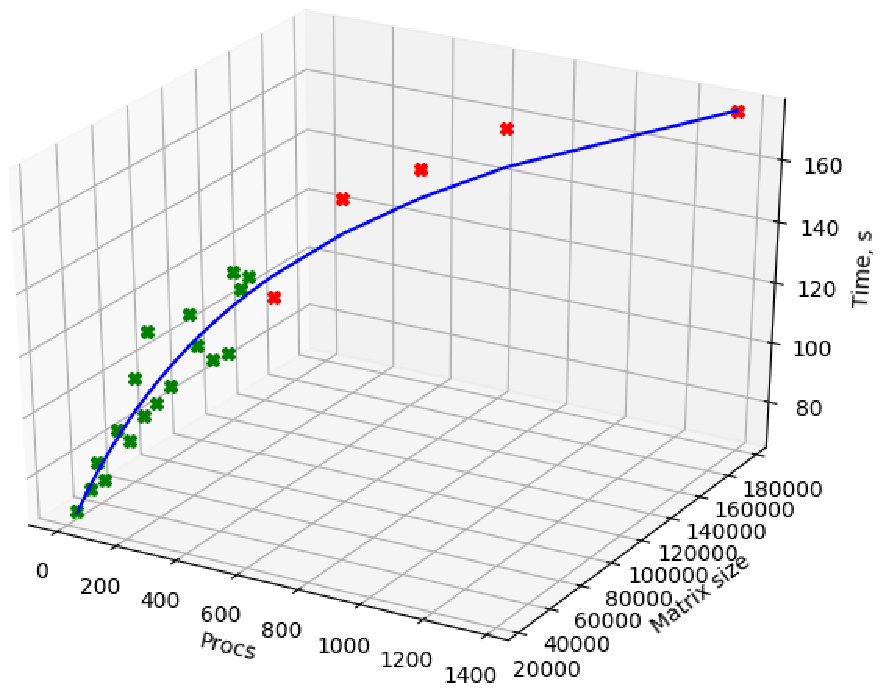
\includegraphics[width=.9\textwidth]{./images/aa}%{./images/fig_hpl_k3}
						\caption{Аппроксимирующая функция предсказаний времени, HPL}
						\label{figure_HPL_C_3}
					\end{figure}
		 			\begin{table}
			 			\captionsetup{font=tiny, labelfont=tiny}
			 			\tiny
							\begin{tabularx}{\textwidth}{|X|X|X|X|X|X|}%{|p{0.3cm}||p{0.3cm}|p{0.3cm}|p{0.3cm}|p{0.3cm}|p{0.3cm}|}
								\hline
								  PN &  225 &  400 &  576 &  784 & 1369 \\ \hline
								Mean & 5,09 & 7,17 & 3,74 & 4,43 & 2,95 \\ \hline
							\end{tabularx}
						\caption{Относительные ошибки предсказаний, усреднённые по количеству процессов, HPL}
					\end{table}
				\end{column}
	 		\end{columns}
	 	\end{frame}
	 	% \begin{frame}
	 	% 	\small
			% \frametitle{\insertsection}
	 	% 	\framesubtitle{\insertsubsection}
	 	% 	\begin{columns}
	 	% 		\begin{column}{.5\textwidth}
	 	% 			\begin{itemize}[label = \(\bullet\)]
			% 	 		\item HPL — тест производительности вычислительной системы.
			% 	 		%, на основе результатов которого формируется современный список TOP500 лучших суперкомпьютеров в мире.
			% 	 		Суть теста заключается в решении плотных систем линейных алгебраических уравнений, используя LU факторизацию.
			% 	 		\item Сложность алгоритма \(\mathcal{O}(N^3)\)
			% 	 		\item Количество операций чтения/записи \(\mathcal{O}(N^2)\).
			% 	 		\end{itemize}
			% 	 			\begin{table}
			% 	 			\captionsetup{font=tiny, labelfont=tiny}
			% 	 				\tiny
			% 					\begin{tabular}{|r||p{0.3cm}|p{0.3cm}|p{0.3cm}|p{0.3cm}|p{0.3cm}|}
			% 						\hline
			% 						  PN &  225 &  400 &  576 &  784 & 1369 \\ \hline
			% 						mean & 5,09 & 7,17 & 3,74 & 4,43 & 2,95 \\ \hline
			% 					\end{tabular}
			% 				\caption{Относительные ошибки предсказаний, усреднённый по количеству процессов, HPL}
			% 				\end{table}	
	 	% 		\end{column}
	 	% 		\begin{column}{.5\textwidth}
					
			% 		\begin{table}
			% 			\captionsetup{font=tiny, labelfont=tiny}
			% 			\tiny
			% 			\begin{tabular}{|c|c|c|c|}
			% 				\hline
			% 				\multicolumn{4}{|c|}{\(C_1\)}     \\ \hline
			% 				  PN &   PS & RE\_time & RE\_perf \\ \hline
			% 				 225 & 60,8 &     7,58 & 6,82     \\ \hline
			% 				 400 & 73,7 &     1,79 & 1,90     \\ \hline
			% 				 576 & 83,2 &     0,37 & 0,45     \\ \hline
			% 				 784 & 92,2 &     0,12 & 0,09     \\ \hline
			% 				1369 &  111 &     0,16 & 0,07     \\ \hline
			% 				\hline
			% 				\multicolumn{4}{|c|}{\(C_2\)}      \\ \hline
			% 				  PN &    PS & RE\_time & RE\_perf \\ \hline
			% 				 225 & 76,65 &     3,82 & 0,82     \\ \hline
			% 				 400 & 92,85 &     7,53 & 16,35    \\ \hline
			% 				 576 & 104,8 &     0,62 & 9,25     \\ \hline
			% 				 784 & 116,1 &     1,42 & 10,59    \\ \hline
			% 				1369 &   140 &    11,35 & 4,41     \\ \hline
			% 				\hline
			% 				\multicolumn{4}{|c|}{\(C_3\)}      \\ \hline
			% 				  PN &    PS & RE\_time & RE\_perf \\ \hline
			% 				 225 & 100,8 &     5,79 & 5,69     \\ \hline
			% 				 400 &   117 &     7,73 & 7,73     \\ \hline
			% 				 576 &   132 &     6,06 & 5,72     \\ \hline
			% 				 784 & 146,3 &     7,42 & 6,95     \\ \hline
			% 				1369 & 176,2 &     0,02 & 1,69     \\ \hline
			% 			\end{tabular}
			% 			\caption{Целевые конфигурации запусков HPL для трёх различных значений констант и значения относительных ошибок предсказания времени и производительности на этих конфигурациях}
			% 			% % Тестовые конфигурации запуска, используемые для вычислений параметров модели, и целевых конфигураций, необходимые для оценки погрешности предсказаний, приведены в таблицах \eqref{test_HPL} и \eqref{target_HPL} соответственно. Коэффициенты \(C_1, C_2, C_3\), определяющие значение отношения количества работы приходящееся на один процесс и количества используемых процессов, из выражения \eqref{weak_sc}, связаны соотношением: \(4 \cdot C_1 = 2 \cdot C_2 = C_3 \), то есть с увеличением на единицу номера коэффициента количество работы на один процесс увеличивается в два раза.
						
			% 			%\label{target_HPL}
			% 		\end{table}
					

			% 	\end{column}
	 	% 	\end{columns}
	 		
	 	% \end{frame}
		\subsection{HPCG}
			\begin{frame}
				\footnotesize
				\frametitle{\insertsection}
		 		\framesubtitle{\insertsubsection}
		 		\begin{columns}[T]
		 			\setlength{\mylen}{0.53\textwidth}
		 			\begin{column}{\mylen}
		 				\begin{itemize}[label = \(\bullet\)]
					 		\item HPCG — альтернативный HPL тест производительности.
					 		\item Сильно выделяется на фоне остальных приложений, так как сложность алгоритма и количество операций чтения/записи \(\mathcal{O}(N)\).
					 	\end{itemize}
					 	\begin{table}
				 			\captionsetup{font=tiny, labelfont=tiny}
				 			\tiny
								\begin{tabularx}{\textwidth}{|X|X|X|X|}
									\hline
								PN	& PS  & RE\_time & RE\_perf \\ \hline
								280 & \multirow{5}{*}{\(PN \cdot 104^3\)} & 0,02     & 0,37     \\ \cline{1-1} \cline{3-4}
								560 &     & 1,56     & 0,80     \\ \cline{1-1} \cline{3-4}
								700 &     & 1,89     & 13,07    \\ \cline{1-1} \cline{3-4}
								980	&     & 2,85     & 19,54    \\ \cline{1-1} \cline{3-4}
								1400 &    & 7,05     & 8,99     \\ \hline
								\end{tabularx}
							\caption{Относительные ошибки предсказаний времени и производительности, HPCG}
						\end{table}
					 			
		 			\end{column}
		 			\begin{column}{\dimexpr\textwidth-\mylen}
			 			\begin{figure}
							\captionsetup{font=tiny, labelfont=tiny}
							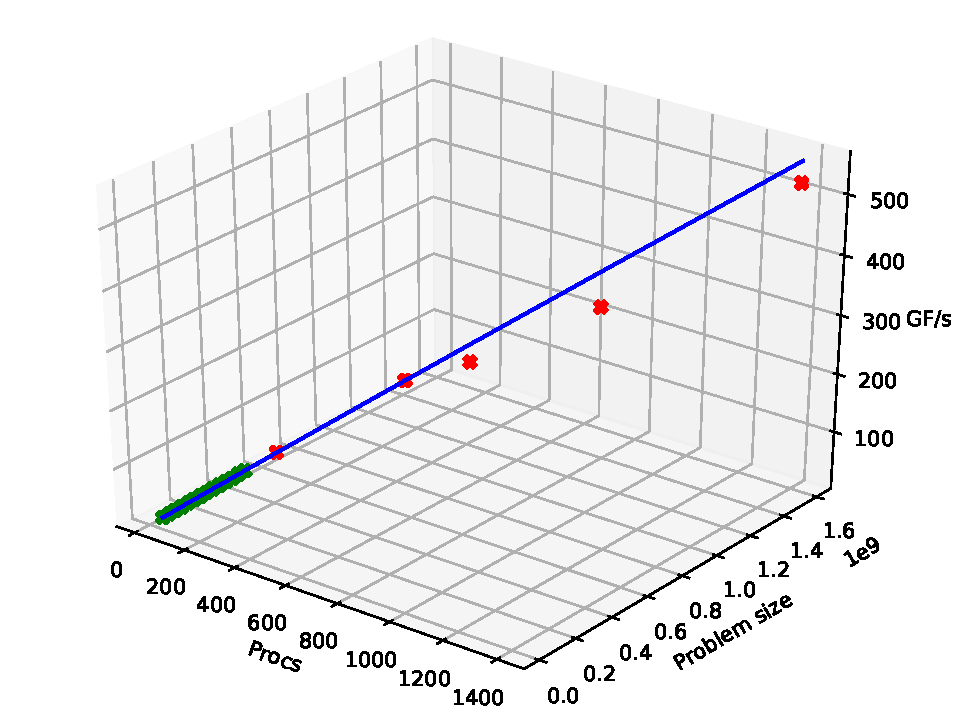
\includegraphics[width=\textwidth]{./images/bbb1}%{./images/fig_hpl_k3}
							\caption{Аппроксимирующая функция предсказаний производительности, HPCG}
						\end{figure}
					\end{column}
		 		\end{columns}
			\end{frame}
		
		\subsection{Алгоритмы матричного умножения, SUMMA}
			% \begin{frame}
			% 	\footnotesize
			% 	\frametitle{\insertsection}
		 % 		\framesubtitle{\insertsubsection}
		 % 		\begin{columns}[T]
		 % 			\setlength{\mylen}{0.45\textwidth}
		 % 			\begin{column}{\mylen}
		 % 				\begin{itemize}[label = \(\bullet\)]
			% 		 		\item SUMMA — алгоритм матричного умножения.
			% 		 		\item Используется в ScaLAPAK и PBLAS.
			% 		 		\item Сложность алгоритма \(\mathcal{O}(N^3)\)
			%  				\item Количество операций чтения/записи \(\mathcal{O}(N^2)\).
			%  				\item \(T_A(N)\:/\:p = const\linebreak\Rightarrow p = N^3\:/\:const\)
			% 		 	\end{itemize}	 			
		 % 			\end{column}
		 % 			\begin{column}{\dimexpr\textwidth-\mylen}
			%  			\begin{figure}
			% 				\captionsetup{font=tiny, labelfont=tiny}
			% 				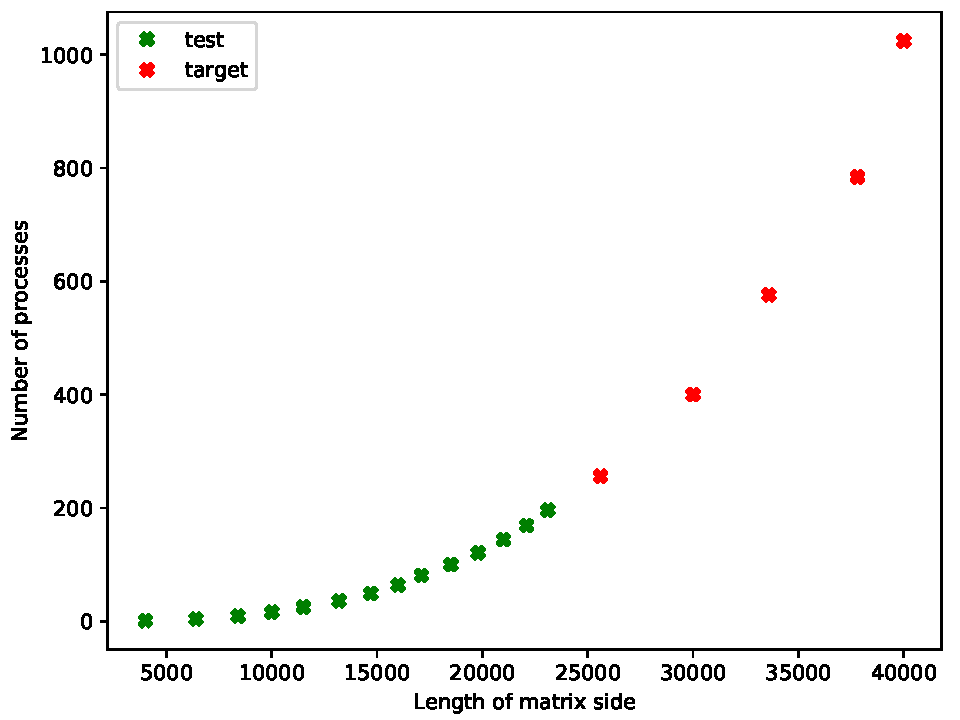
\includegraphics[width=\textwidth]{./images/conf_SUMMA_NEW}%{./images/fig_hpl_k3}
			% 				\caption{Конфигурации запусков матричного умножения по алгоритму SUMMA}
			% 			\end{figure}
			% 		\end{column}
		 % 		\end{columns}
			% \end{frame}
			% \begin{frame}
			% 	\footnotesize
			% 	\frametitle{\insertsection}
		 % 		\framesubtitle{\insertsubsection}
		 % 		\begin{columns}[T]
		 % 			\setlength{\mylen}{0.45\textwidth}
		 % 			\begin{column}{\mylen}
		 % 			\begin{table}
			%  			\captionsetup{font=tiny, labelfont=tiny}
			%  			\tiny
			% 				\begin{tabularx}{\textwidth}{|X|X|X|}
			% 				\hline
			% 				\multicolumn{3}{|c|}{\(C_1\)} \\ \hline
			% 				PN   & PS   & RE\_time        \\ \hline
			% 				225  & 25,6 & 1,95            \\ \hline
			% 				400  & 30   & 3,94            \\ \hline
			% 				576  & 33,6 & 3,01            \\ \hline
			% 				784  & 37,8 & 7,59            \\ \hline
			% 				1024 & 40   & 1,39            \\ \hline
			% 				\end{tabularx}
			% 			\caption{Относительные ошибки предсказаний времени, SUMMA}
			% 		\end{table}
		 				
			% 		 % 	\begin{table}
			% 	 	% 		\captionsetup{font=tiny, labelfont=tiny}
			% 	 	% 		\tiny
			% 			% 		\begin{tabularx}{\textwidth}{|X|X|X|}
			% 			% 			\hline
			% 			% 			PN   & RE\_time & RE\_perf \\ \hline
			% 			% 			280	 & 0,02     & 0,37     \\ \hline
			% 			% 			560	 & 1,56     & 0,80     \\ \hline
			% 			% 			700	 & 1,89     & 13,07    \\ \hline
			% 			% 			980	 & 2,85     & 19,54    \\ \hline
			% 			% 			1400 & 7,05     & 8,99     \\ \hline
			% 			% 		\end{tabularx}
			% 			% 	\caption{Относительные ошибки предсказаний времени и производительности HPCG}
			% 			% \end{table}	 			
		 % 			\end{column}
		 % 			\begin{column}{\dimexpr\textwidth-\mylen}
			%  			\begin{figure}
			%  				\captionsetup{font=tiny, labelfont=tiny}
			% 				\centering
			% 				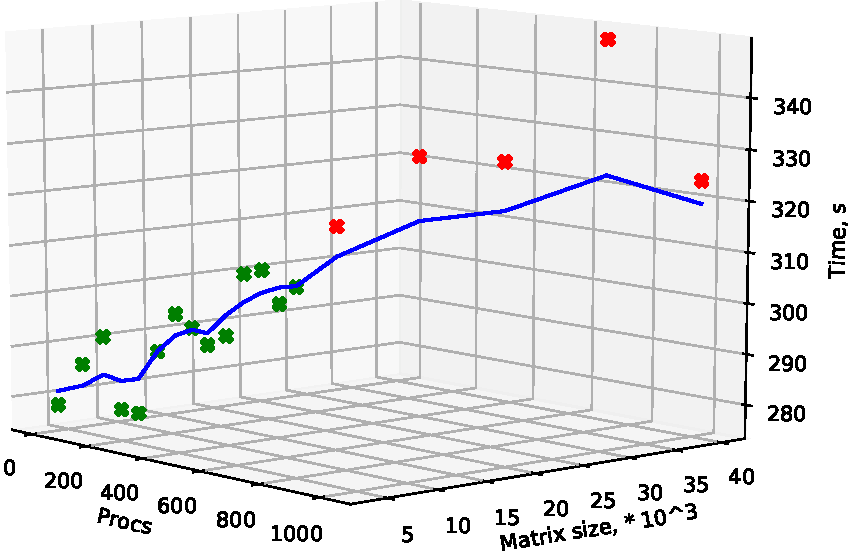
\includegraphics[width=\textwidth]{./images/ccc}
			% 				\caption{Аппроксимирующая функция для слабой масштабируемости матричного умножения по алгоритму SUMMA}
			% 				\label{graph_SUMMA}
			% 			\end{figure}
			% 		\end{column}
		 % 		\end{columns}
			% \end{frame}
			\begin{frame}
				\footnotesize
				\frametitle{\insertsection}
		 		\framesubtitle{\insertsubsection}
		 		\begin{columns}[T]
		 			\setlength{\mylen}{0.5\textwidth}
		 			\begin{column}{\mylen}
		 				\begin{figure}
							\captionsetup{font=tiny, labelfont=tiny}
							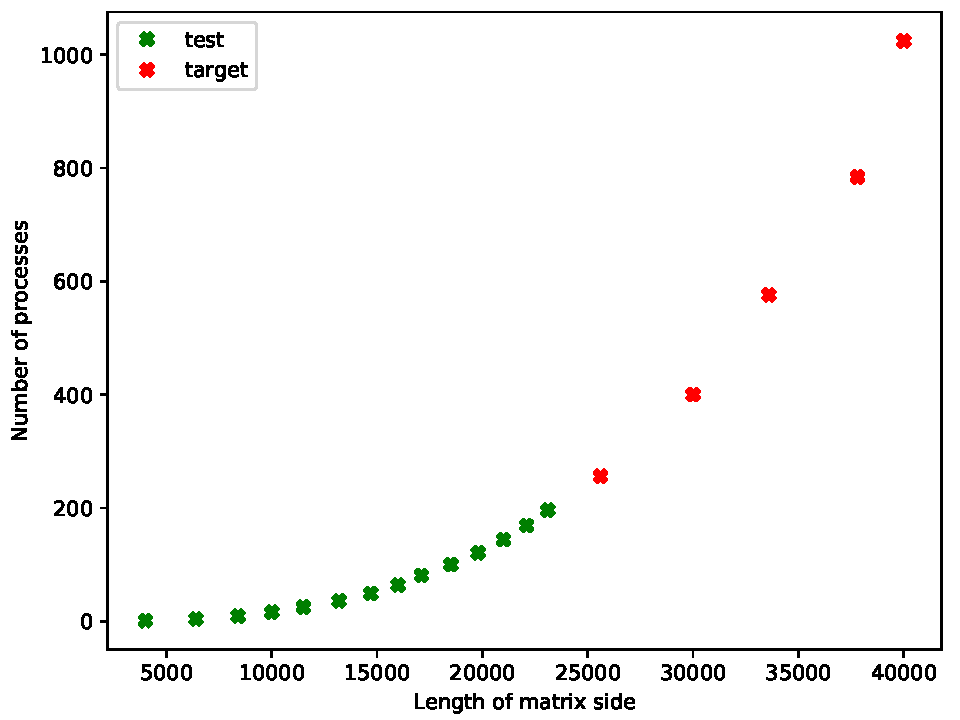
\includegraphics[width=.83\textwidth]{./images/conf_SUMMA_NEW}%{./images/fig_hpl_k3}
							\caption{Конфигурации запусков матричного умножения по алгоритму SUMMA}
						\end{figure}
						\begin{itemize}[label = \(\bullet\)]
					 		\item SUMMA — алгоритм матричного умножения.
					 		\item Используется в ScaLAPAK и PBLAS.
					 		\item Сложность алгоритма \(\mathcal{O}(N^3)\)
			 				\item \(\Rightarrow p = N^3\:/\:const\)
					 	\end{itemize}
					 % 	\begin{table}
				 	% 		\captionsetup{font=tiny, labelfont=tiny}
				 	% 		\tiny
						% 		\begin{tabularx}{\textwidth}{|X|X|X|}
						% 			\hline
						% 			PN   & RE\_time & RE\_perf \\ \hline
						% 			280	 & 0,02     & 0,37     \\ \hline
						% 			560	 & 1,56     & 0,80     \\ \hline
						% 			700	 & 1,89     & 13,07    \\ \hline
						% 			980	 & 2,85     & 19,54    \\ \hline
						% 			1400 & 7,05     & 8,99     \\ \hline
						% 		\end{tabularx}
						% 	\caption{Относительные ошибки предсказаний времени и производительности HPCG}
						% \end{table}	 			
		 			\end{column}
		 			\begin{column}{\dimexpr\textwidth-\mylen}
			 			\begin{figure}
			 				\captionsetup{font=tiny, labelfont=tiny}
							\centering
							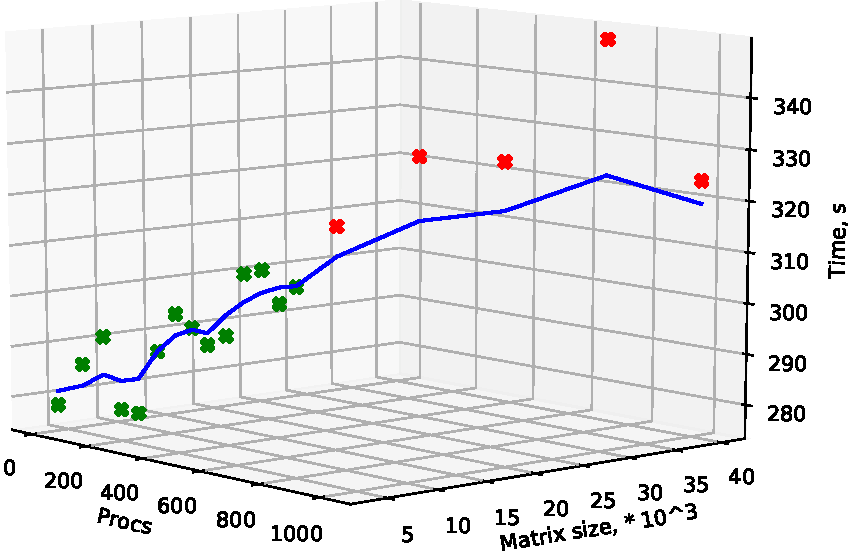
\includegraphics[width=0.9\textwidth]{./images/ccc}
							\caption{Аппроксимирующая функция предсказаний времени, SUMMA}
							\label{graph_SUMMA}
						\end{figure}
						\begin{table}
			 			\captionsetup{font=tiny, labelfont=tiny}
			 			\tiny
							\begin{tabularx}{\textwidth}{|X|X|X|}
							\hline
							PN   & PS   & RE\_time        \\ \hline
							225  & 25,6 & 1,95            \\ \hline
							400  & 30   & 3,94            \\ \hline
							576  & 33,6 & 3,01            \\ \hline
							784  & 37,8 & 7,59            \\ \hline
							1024 & 40   & 1,39            \\ \hline
							\end{tabularx}
						\caption{Относительные ошибки предсказаний времени, SUMMA}
					\end{table}
					\end{column}
		 		\end{columns}
			\end{frame}
		\subsection{Алгоритмы матричного умножения, DNS}
			% \begin{frame}
			% 	\footnotesize
			% 	\frametitle{\insertsection}
		 % 		\framesubtitle{\insertsubsection}
		 % 		\begin{columns}[T]
		 % 			\setlength{\mylen}{0.5\textwidth}
		 % 			\begin{column}{\mylen}
		 % 				\begin{figure}
			% 				\captionsetup{font=tiny, labelfont=tiny}
			% 				%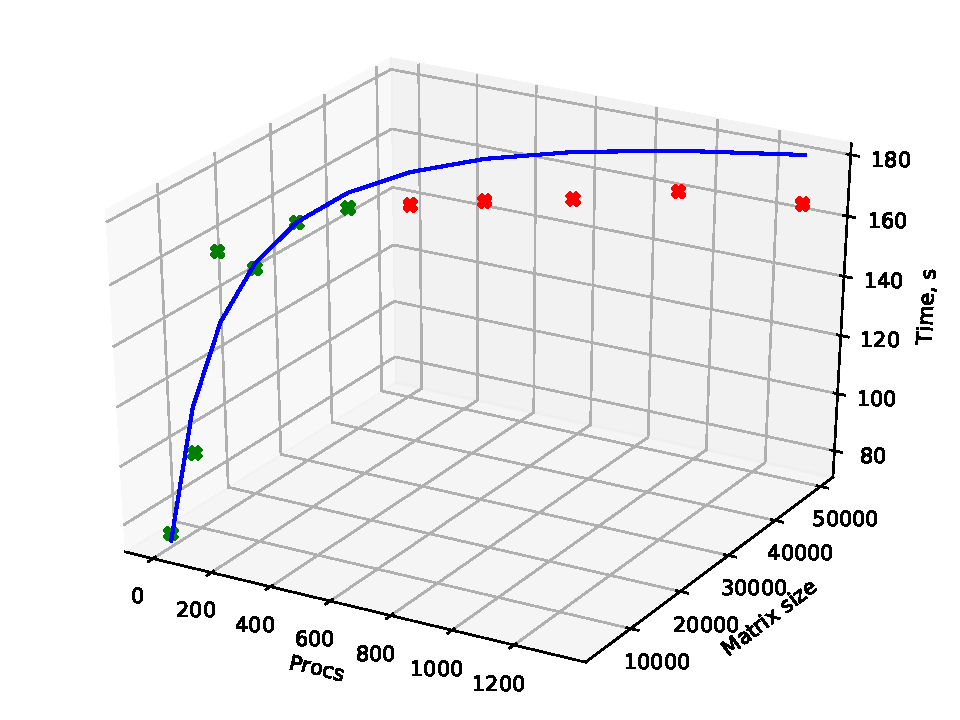
\includegraphics[width=.9\textwidth]{./images/graph_C_1_DNS}%{./images/fig_hpl_k3}
			% 				\caption{AAA}
			% 			\end{figure}
			% 			\begin{itemize}[label = \(\bullet\)]
			% 		 		\item DNS — алгоритм матричного умножения.
			% 		 		\item Сложность алгоритма \(\mathcal{O}(N^3)\)
			% 		 	\end{itemize}
			% 		 % 	\begin{table}
			% 	 	% 		\captionsetup{font=tiny, labelfont=tiny}
			% 	 	% 		\tiny
			% 			% 		\begin{tabularx}{\textwidth}{|X|X|X|}
			% 			% 			\hline
			% 			% 			PN   & RE\_time & RE\_perf \\ \hline
			% 			% 			280	 & 0,02     & 0,37     \\ \hline
			% 			% 			560	 & 1,56     & 0,80     \\ \hline
			% 			% 			700	 & 1,89     & 13,07    \\ \hline
			% 			% 			980	 & 2,85     & 19,54    \\ \hline
			% 			% 			1400 & 7,05     & 8,99     \\ \hline
			% 			% 		\end{tabularx}
			% 			% 	\caption{Относительные ошибки предсказаний времени и производительности HPCG}
			% 			% \end{table}	 			
		 % 			\end{column}
		 % 			\begin{column}{\dimexpr\textwidth-\mylen}
			%  			\begin{figure}
			%  				\captionsetup{font=tiny, labelfont=tiny}
			% 				\centering
			% 				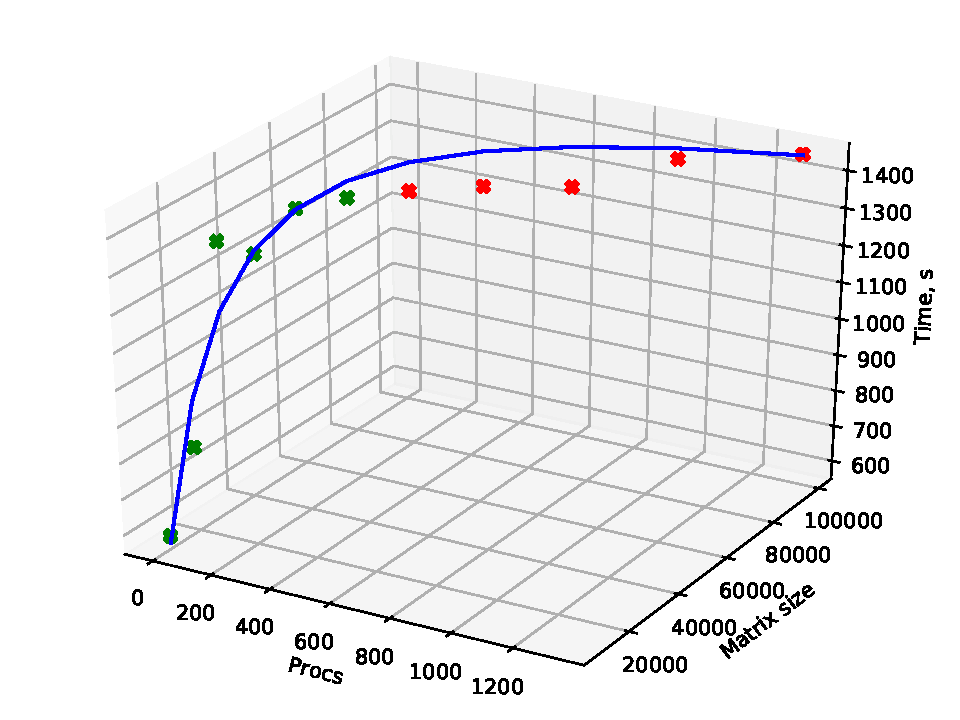
\includegraphics[width=.9\textwidth]{./images/graph_C_2_DNS}
			% 				\caption{Аппроксимирующая функция для слабой масштабируемости матричного умножения по алгоритму SUMMA}
			% 				\label{graph_SUMMA}
			% 			\end{figure}
			% 			\begin{table}
			% 	 			\captionsetup{font=tiny, labelfont=tiny}
			% 	 			\tiny
			% 					\begin{tabularx}{\textwidth}{|X||X|X||X|X|}
			% 					\hline
			% 			             & \multicolumn{2}{|c|}{\(C_1\)} & \multicolumn{2}{|c|}{\(C_2\)} \\ \hline
			% 			        PN   & PS   & RE\_time & PS & RE\_time          \\ \hline
			% 			        343  & 31,5 & 6,55     & 63 & 5,66              \\ \hline
			% 			        512  & 36   & 8,42     & 72 & 6,84              \\ \hline
			% 			        729  & 40,5 & 9,35     & 81 & 7,85              \\ \hline
			% 			        1000 & 45   & 7,94     & 90 & 1,94              \\ \hline
			% 			        1331 & 49,5 & 9,63     & 99 & 0,19              \\ \hline
			% 					\end{tabularx}
			% 				\caption{Относительные ошибки предсказаний времени, SUMMA}
			% 			\end{table}
			% 		\end{column}
		 % 		\end{columns}
			% \end{frame}

			\begin{frame}
				\footnotesize
				\frametitle{\insertsection}
		 		\framesubtitle{\insertsubsection}
				\begin{columns}[T]
					\setlength{\mylen}{0.5\textwidth}
					\begin{column}{\mylen}
						\begin{figure}
							\captionsetup{font=tiny, labelfont=tiny}
							\centering
							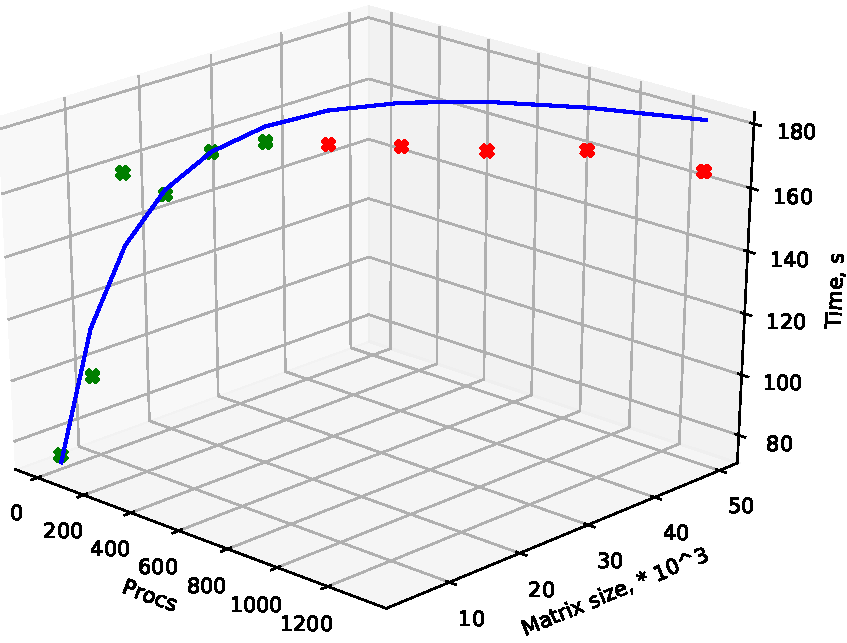
\includegraphics[width=.7\textwidth]{./images/dns_k2}
							%\caption{Аппроксимирующая функция для слабой масштабируемости матричного умножения по алгоритму SUMMA}
						\end{figure}
					\end{column}
					\begin{column}{\dimexpr\textwidth-\mylen}
						\begin{figure}
							\captionsetup{font=tiny, labelfont=tiny}
							\centering
							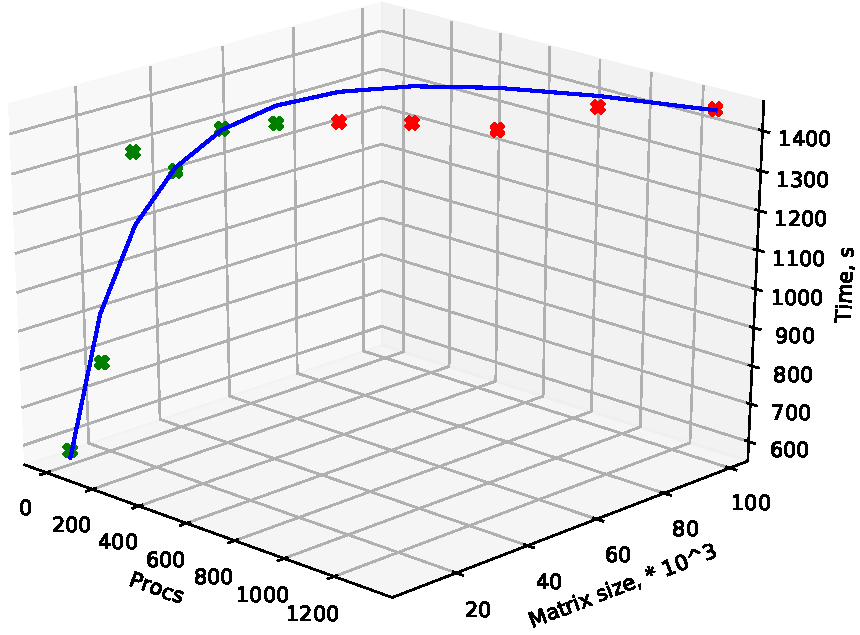
\includegraphics[width=.7\textwidth]{./images/dns_k1}
							%\caption{Аппроксимирующая функция для слабой масштабируемости матричного умножения по алгоритму SUMMA}
						\end{figure}
					\end{column}
				\end{columns}
				\begin{figure}
					\captionsetup{font=tiny, labelfont=tiny}
					\centering
					\caption{Аппроксимирующие функции предсказаний времени для двух различных значений констант, DNS}
				\end{figure}
				\begin{columns}[T]
					\setlength{\mylen}{0.4\textwidth}
					\begin{column}{\mylen}
						\begin{itemize}[label = \(\bullet\)]
					 		\item DNS — алгоритм матричного умножения.
					 		\item Сложность алгоритма \(\mathcal{O}(N^3)\)
					 		\item Всего 6 тестовых конфигураций
					 	\end{itemize}
					\end{column}
					\begin{column}{\dimexpr\textwidth-\mylen}
						\begin{table}
				 			\captionsetup{font=tiny, labelfont=tiny}
				 			\tiny
								\begin{tabularx}{\textwidth}{|X|X|X||X|X|}
								\hline
						             & \multicolumn{2}{c||}{\(C_1\)} & \multicolumn{2}{c|}{\(C_2\)} \\ \hline
						        PN   & PS   & RE\_time & PS & RE\_time          \\ \hline
						        343  & 31,5 & 6,55     & 63 & 5,66              \\ \hline
						        512  & 36   & 8,42     & 72 & 6,84              \\ \hline
						        729  & 40,5 & 9,35     & 81 & 7,85              \\ \hline
						        1000 & 45   & 7,94     & 90 & 1,94              \\ \hline
						        1331 & 49,5 & 9,63     & 99 & 0,19              \\ \hline
								\end{tabularx}
							\caption{Относительные ошибки предсказаний времени, DNS}
						\end{table}
					\end{column}
				\end{columns}
			\end{frame}
		\subsection{Graph500}
		\begin{frame}
			\frametitle{\insertsection}
			\framesubtitle{\insertsubsection}
			\begin{itemize}[label = \(\bullet\)]
				\item Graph500: BFS и SSSP.
				\item Сложность алгоритмом определяется через количество вершин и рёбер графа \(\mathcal{O}(V + E)\).
				\item Выражая сложность через параметры запуска scalefactor и edgefactor, получим: \(V + E = 2^{SC} + EF \cdot 2^{SC} = 2^{SC} \cdot (1 + EF) \)
				\item Среднее значение относительных ошибок предсказания времени - 13,28\%, производительности - 13,22\%.
				\item Тестовые конфигурации выбираются так, чтобы удовлетворять \(T_A(N)\:/\:p = const\), но не всегда возможно обеспечить строгое равенство \(\Rightarrow\) приходится округлять параметры запусков \(\Rightarrow\) провалы и всплески значений динамических характеристик \(\Rightarrow\) неточные предсказания.
			\end{itemize}

		\end{frame}
	\section{Результаты}
		\begin{frame}
			\frametitle{\insertsection}
			\footnotesize
			%\framesubtitle{\insertsubsection}
			\begin{figure}
				\captionsetup{font=tiny, labelfont=tiny}
				\centering
				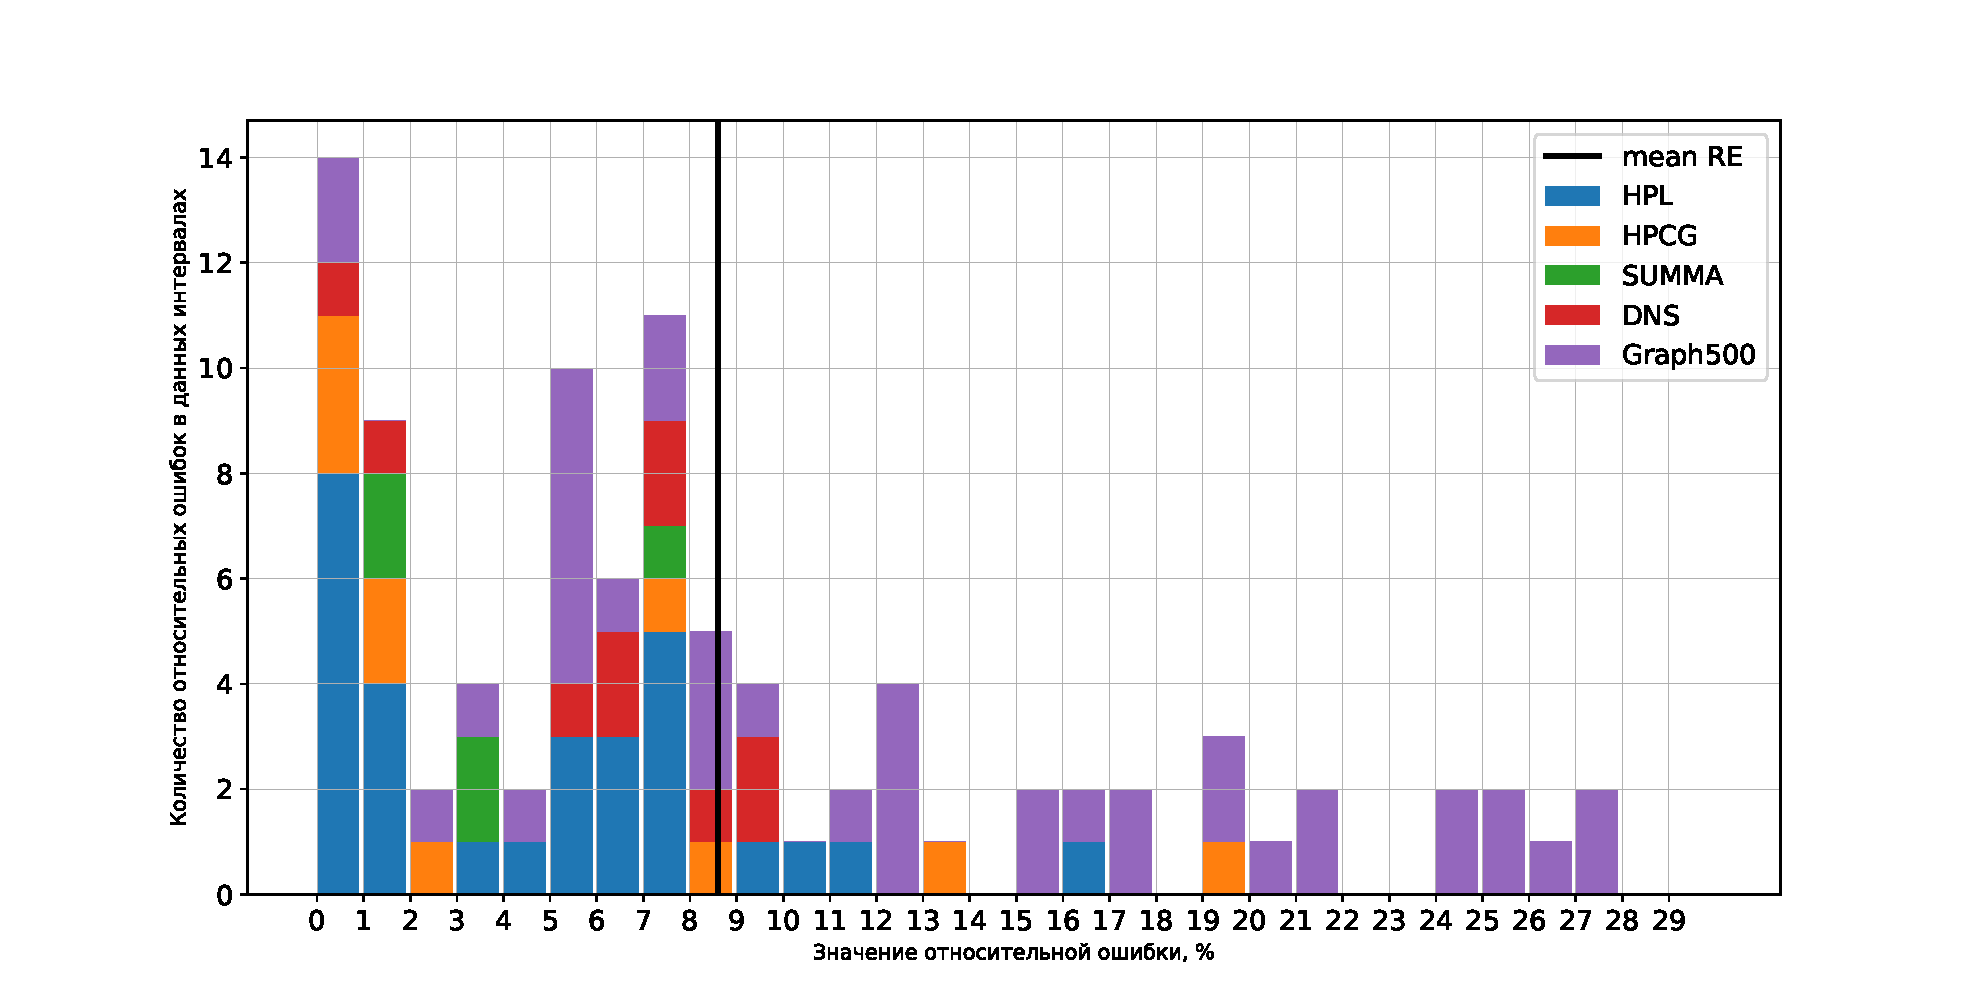
\includegraphics[width=\textwidth]{./images/RE_graph}
				\caption{Относительные ошибки предсказаний на всех конфигурациях всех рассматриваемых приложений}
			\end{figure}
			
			\begin{itemize}[label = \(\bullet\)]
			\item Среднее значение относительных ошибок - 8,6\% (HPL - 4,9\%, HPCG - 5,6\%, SUMMA - 3,6\%, DNS - 6,4\%, Graph500 - 13,2\%)

			\end{itemize}
		\end{frame}
		\begin{frame}
			\frametitle{\insertsection}
			%\footnotesize
			%\framesubtitle{\insertsubsection}
			\begin{itemize}[label = \(\bullet\)]
			\item Разработан метод, предсказывающий слабую масштабируемость суперкомпьютерных приложений на основе экспериментальных данных со средней относительной ошибкой по всем смотренным приложениям равной 8,6\%.
			\item Выполнена проверка применимости метода на различных приложениях (HPL, HPCG, матричных алгоритмов умножения SUMMA и DNS, Graph500) на суперкомпьютере "<Ломоносов-2">.
			\end{itemize}
		\end{frame}



\end{document}



% \begin{frame}
% 	\frametitle{\insertsection}
% 	\framesubtitle{\insertsubsection}

% \end{frame}



